\setlength{\parindent}{0em}
\setlength{\parskip}{1em}
\chapter{Introduction}

Linux distributions are built upon packages that provide software to their users. It is these
packages that make particular distribution different or similar to another one. All these packages require
maintenance, in this case, the distribution is developed commercially, as well as is developed by the community.
The fact that the whole system is stable and comfortable to use is a result of the good work of
maintainers who work together to ensure that all packages are working and their
requirements are met.

Efficient maintenance requires accurate information, which maintainers get from multiple sources
and use many tools to retrieve. For example, which packages depend on their packages, and thus which
maintainers should they communicate with when encountering disturbing changes? Often the information
is not easy to acquire and slows down developers by forcing them to manually search through different
places. To solve this problem, a new tool that can store and filter any information about
packages is required as no other exists at the moment.

RPQR is an originally proposed tool that is supposed to make maintainers' life easier by allowing them to describe how
to acquire the data only once and then be able to retrieve it on demand. It is flexible
enough to store any new kind of data and to search packages based on a combination of any of them while
also providing the option to accelerate queries by making specialized commands.
RPQR also lets users build a cache which makes further queries faster and thus saves time while
doing everyday work.

The tool can be directly used by other projects through provided API. It can also be used
by a user as any other command-line project. Users are also able to visualize their
results for a faster understanding of the results.

\chapter{Theory and current state}
While crucial information about an RPM package is stored directly inside it within the header section,
additional information as who maintains it or which bugs are currently known has to be searched
in external sources of information. This chapter describes RPM packages and technologies which
currently exist for working with them. Then there is a description of other subjects which are needed
to successfully design and implement the RPQR project.

\section{RPM package}
RPM packages have their file format\cite{RPMFileFormat}. It is composed of four parts with their specific purposes.
The parts are (i)lead, (ii)signature, (iii)header and (iv)archive. Here are described and explained all parts
relevant to the RPQR project.

\subsection*{The lead}
The lead is the first part of the RPM package. It contains the magic number and version of the RPM file format.
It also contains whether the package type is binary or source and other information relevant
to a system using it. The difference between binary and source packages is that the source package contains
source code from which software can be built or the whole downloaded project, while the binary package
contains the actual software. The lead is no longer used internally by RPM because of its
inflexibility and is noted here only for completeness of file format description.

\subsection*{The signature}
The signature is allowing package integrity and optionally authenticity to be verified. It holds
little purpose for RPQR but it is important because DNF uses it and RPQR is using DNF API.

\subsection*{The header}
The header is the most interesting part from the perspective of the RPQR project because it contains
detailed crucial information about the package. It is composed of tags that describe different
aspects of the bundled software. Examples of these tags can be \mbox{\textit{RPMTAG\_VERSION}}
specifying a version of the package or \textit{RPMTAG\_RELEASE} which specifies what release of
this version this is. The header is parsed by software that is making the metadata structure of RPM
repositories and this structure is then used by the DNF package manager to find appropriate
packages that the user needs.

\begin{lstlisting}
00001198  8e ad e8 01 00 00 00 00  00 00 00 3e 00 00 0f dd  |...........>....|
\end{lstlisting}

The first 16 bytes of the header part are describing the attributes of this header. Three bytes are
the magic number identifying the header, one byte says that the header conforms to version 1 of the specification.
Four other bytes are reserved. Then there is a count of entries stored in this header
(00 00 00 3e to decimal is 62). The last four bytes mean how many bytes are stored in this structure
(00 00 0f dd to decimal is 4061).

\begin{lstlisting}
000011c8  00 00 03 e8 00 00 00 06  00 00 00 02 00 00 00 01  |................|
\end{lstlisting}

For the best example, we will describe the name tag. 00 00 03 e8 identifies the presence of
a name tag and 00 00 00 06 says that value is a string. 00 00 00 02 means that the value
is located 2 bytes after the start of the store and 00 00 00 01 indicates that there is
just one value, which is the only allowed possibility for string value stored in the header.

The store is composed of values after each other that are distinguished only by their respective offsets.

\subsection*{The archive}
The archive is a set of files and folders compressed with a compression algorithm. Its integrity
can be verified with the specified signature.

\section{RPM repository}
RPM repositories are directory structures that contain RPM packages and metadata which are needed
to quickly locate packages that the user needs. Metadata are created by \textit{createrepo} \cite{RPMRepository}
utility and accessed by the DNF package manager. 

\subsection*{Repodata}
Every RPM repository contains a folder \textit{repodata} which contains data about the contents of the
repository. There is a file \textit{repomd.xml} containing XML structure indicating where should
package manager look for databases with information about packages.

Important databases:
\begin{itemize}
  \item \textbf{primary} database which specifies all crucial information about each package as of version, description, or file list.
  \item \textbf{other} database which contains other less important information e.g. changelog of a~package
\end{itemize}

\section{Package managers}
Working with RPM packages can be done with multiple tools. Their general responsibility is to recognize
package dependencies and being able to install or uninstall software contained in the package.
Most frequently used are RPM package manager and DNF package manager (successor of the old
YUM package manager).

\subsection*{RPM package manager}
RPM package manager supports more low-level operations with packages than DNF does \cite{RPMPackageManager}. It allows
to build the source of a project according to specfile and create distributable packages. More of the
important operations are also reading the metadata and verification of installed software, in
case it is not working properly. Installation of dependencies would have to be handled by a user
manually so the rpm utility is not often used by end-users of the systems.

\subsection*{YUM package manager}
Yum package manager is historically the first manager that allowed easy downloading of packages
from remote repositories and handling their dependencies \cite{YUMPackageManager}. It is currently deprecated and has been
replaced by DNF. Reasons for deprecation and replacement were that YUM was not properly documented,
it was not ready for a switch to Python3, and the algorithm for dependency resolution was not strong enough
to handle all problems that withstand in modern RPM-based Linux distributions.

\subsection*{DNF package manager}
DNF package manager is a successor of the older YUM package manager \cite{DNFPackageManager}. It allows users to install and remove software
on the system comfortably by handling all of the operations that are needed to retrieve package dependencies
and resolve any possible conflicts. A~very often used feature is also system upgrades, when
DNF can migrate a system from old versions of distribution to new ones. A~very important fact
that needs to be stated is that DNF provides Python API which can be used by other projects to retrieve metadata
from repositories and distinguish them.

DNF is the only tool that is currently able to query repositories for metadata that are specified
in packages. An example of a frequently used query is:

\textit{\$ dnf repoquery -{}-whatprovides /usr/bin/bash}

This command issues that DNF should execute command \textit{repoquery} filtering by tag \mbox{\textit{provides}}
and find all packages that provide file \textit{/usr/bin/bash}. DNF can search for packages based on
attributes that are supplied within the package, but it is not able to retrieve additional information
or query based on complex relationships. It is not its job to resolve more difficult queries and
it would be wrong to force it to by extending its capabilities.

\section{DNF API}
DNF provides Python API through which developers can interact with repositories and retrieve information.
At first, an instance of \textit{Base} class has to be created and then specify repositories from which
metadata should be retrieved. Call to \textit{fill\_sack} method after that will load the metadata
and API can then execute queries that the DNF tool supports.

Example of how is dnf API used in RPQR project:
\begin{lstlisting}
  base = dnf.Base()
  for (name, url) in self.repositories:
      base.repos.add_new_repo(name, base.conf, baseurl=[url])
  base.fill_sack(load_system_repo=False, load_available_repos=True)
  return base.sack.query().available()
\end{lstlisting}

\section{Storing techniques and query language}
As was stated before, it is crucial to choose the right technologies to store package metadata in
such a format that they can be read by a human reader while also easily parsable and serializable.
This section will describe possible formats. Another part will explain the existing query
languages that could be used for RPQR queries and their pros and cons in the context of describing
package metadata.

\subsection*{Data structures}
While RPM repositories store metadata as a list in XML format or \textit{sqlite} database, for use cases that
are oriented about relationships between packages list does not have to be appropriate data
structure for internal representation of package metadata.

\newpage

\begin{itemize}
  \item List
    \subitem Pros:
    \subsubitem Easy to work with Python
    \subsubitem Simple algorithms to process its members
    \subitem Cons:
    \subsubitem Bad handling of relationship representation
  \item Dictionary
    \subitem Pros:
    \subsubitem Faster accessing of members
    \subitem Cons:
    \subsubitem Forcing packages to be identified by the same attribute
  \item Graph
    \subitem Pros:
    \subsubitem Great representation of relationships between packages
    \subsubitem Fast algorithms for searching and filtration
    \subitem Cons:
    \subsubitem More complex algorithms for processing of nodes
    \subsubitem To filter packages according to attributes, dictionary or list is still needed
                since there is no package that we could consider as the proper root of the graph.
\end{itemize}

\subsection*{Data formats}
\label{sec:dataformats}
An appropriate data format needs to be chosen for storing data. Currently, many massively
used formats could be suitable for the RPQR use case. The data format should be chosen accordingly to
how much readability it can provide for a human developer and whether it can be used within versioning
repositories such as git or mercury.

\subsubsection*{XML}
Extensible markup language\cite{XMLFormat} is used by \textit{repocreate} utility which is parsing package metadata and creating
their collections for package managers. It is natively supported by Python and relatively easy to
read. XML uses tags to distinguish individual elements of serialized data. Its advantage
is that it supports various encodings and even can contain comments so some things in serialized
data could have additional explanations when needed.

\newpage

Example of XML data:
\begin{lstlisting}
  <?xml version="1.0" encoding="UTF-8"?>
  <element>
      <innerElement>
        Example text
      </innerElement>
      <!-- Explanation comment -->
  </element>
\end{lstlisting}

\subsubsection*{JSON}
JavaScript Object Notation\cite{JSONFormat} is a widely used format for data serialization which represents objects
with pairs of named attributes and their values. One of the big advantages is that it also natively
supports arrays and consists of minimal syntax which allows most data to be stored and transferred
with less required space. Unfortunately, there is no support for comments but the readability of JSON
data is generally good so they are not needed in most cases.

Example of JSON data:
\begin{lstlisting}
  {"Element":{
    "InnerElement": "Example text"
    }
  }
\end{lstlisting}

\subsubsection*{YAML}
YAML\cite{YAMLFormat} Ain't Markup Language is a data format used by many applications for configuration and data
transfer. YAML used JSON as a basis for its version 1.2 and it is accepting JSON as its subset.
The interesting about this format is that unlike JSON it supports comments and extensible data types.
Strings in YAML can be also specified without the starting and ending quotation marks. Individual
attributes of objects are distinguished by name and indentation by a style that is similar to Python. While
YAML data sets are generally smaller than JSON, the number of additional syntax features makes
their parsers more complex and thus it inevitably takes more time to load them.
\newpage

Example of YAML data:
\begin{lstlisting}
element:
  InnerElement: Example text
\end{lstlisting}

\subsubsection*{Pickle}
For completeness here is mentioned even Python pickle format\cite{PickleFormat} for object serialization. Because
it is binary it can be parsed more quickly and support the additional acceleration of RPQR execution.
There is an issue with the execution of arbitrary code when parsing pickle structures which does not
occur in previously mentioned formats. Unlike the previous formats, it is not human-readable
and thus unfortunately not appropriate to be used for package data structures that should be accessible
by different tools.
There is no example because it would not make sense to show binary data.

\subsection*{Query languages}
For purposes of the RPQR project, there needs to be a specification on how to describe queries. Currently,
there are many approaches. In this section, there will be a description of some of them and their features
which could prove useful for selecting packages and their attributes.

\subsubsection*{SQL}
Structured Query Language\cite{SQL} is a domain-specific language that is widely used to interact with
relational databases. SQL can select records based upon their attributes and relations but
is not capable of describing complex recursive queries about graphs. Another caveat is that for a Python
application, using standard Python libraries, to be able to use SQL, it would need to hold an instance of \textit{sqlite} database in memory and
that could prove to be an unnecessary overhead\footnote{Resources required to perform an operation} that could slow execution down.

Example of SQL query:
\textit{SELECT * FROM table WHERE id = 3}

\subsubsection*{GraphQL}
GraphQL\cite{GraphQL} is an open-source query language that allows developers to implement their interpretation
of individual query parameters. It is used in REST APIs to allow client applications to retrieve data
effectively from a server without it having to transfer any unnecessary data. Its flexibility is
a great advantage, but queries are not as readable as they would be in SQL language.

\subsection*{Cypher query language}
Cypher query language is an implementation of \textit{opencypher} specification. It is meant to work with
the neo4j graph database and is developed for such a purpose. For an application to be able to get the advantage
of cypher, it needs to use the neo4j database which can result in too big an overhead for utilities
designed with one specific purpose in mind.

Example of Cypher query language:

\textit{MATCH (peter: employee {name: 'Peter Parker'}) RETURN peter}

Example of GraphQL query:

\begin{lstlisting}
  {
    table(where: {id: {_eq: 3}}) {
      id
      name
      age
    }
  }
\end{lstlisting}

\subsubsection*{Domain specific language on Python}
Creating query language is always an option and it holds enormous power in the ability to
bend the language to the specific purpose that the RPQR project needs. Problem is that developing
and maintaining language takes time and energy. For a language to be functional, RPQR would
need to implement its components like scanner, parser, and interpreter. In the essence,
a domain-specific language for RPQR would need to be relatively simple. There is a requirement
to interpret statements which result is always a set of nodes that represent packages. These
statements consist of commands that take values and other statements as arguments and operators
which realize basic set operations as is union or intersection.

Example of how RPQR language could look:

WHATDEPENDSON('libyang', 3) \& WHATDEPENDSON('libgcc', 3)

\newpage

Components that are needed for interpretation of RPQR language:
\begin{itemize}
  \item \textbf{Scanner}

  The scanner is used to convert the source text of the language to tokens for further processing by the parser.
  Its crucial part is a finite state machine that reacts to characters in input and recognizes lexical
  tokens. The scanner is also able to tell a~user when some lexical error occurs and the query needs to be
  changed for it to be valid.
  
  \item \textbf{Parser}
  
  Parser consumes tokens from the scanner and handles the creation of abstract syntactic tree or some other
  internal representation of source text on input. The parser can recognize syntactic errors
  which occur during parsing and optionally inform the user about them. There are multiple techniques
  for syntactic analysis as Top-Down Parsing or Bottom-Up Parsing, which are algorithms
  how to recognize language units on input. Both of these techniques use models for context-free
  languages such as formal grammar. Formal grammar is a list of rules which are used to check
  whether the input is written in a language or not.

  \item \textbf{Interpreter}
  
  RPQR does not need to translate the query into some other form, it needs to perform it. That is the
  reason why the last part of the RPQR language would be its interpreter. The interpreter inside of RPQR would need to be
  flexible enough for it to be able to accept new commands for searching for packages. Another important thing is using optimizations such as short evaluation to make searching for packages
  as fast as possible.
\end{itemize}

\section{Caching}
Since one of the most time-consuming actions of the current approach to queries about RPM packages is
network communication and transfer of metadata, it is crucial to download all metadata at once at
the start of execution to not need any further downloads. This can be ensured through DNF API by
executing a query to list all packages that are available to install from specified repositories.
DNF package manager uses a very similar approach by downloading all metadata to local storage and
updating it only when the user forces it to or the cache expires.

The question of metadata expiration needs to be handled by the RPQR itself too.

Approach, when metadata is not updated unless the user wants to do so, could save time for
checking of the repository, but the user would be responsible for the consistency of metadata and repository
state, which could prove problematic.

RPQR could stick with the same approach as the DNF. That means rebuilding metadata when they expire.
The problem is that building internal structure and rebuilding cache could be a~very time-consuming
operation, maybe even in a matter of minutes.

The third and maybe the most proper approach is to set the expiration time of metadata to some
longer period. After such a period the time, rebuilding of the cache will not be so important.
Also if no change occurred then it is pointless to rebuild the data and it would be highly useful
to rebuild only parts of internal data structures which do not longer correspond with the actual state
of RPM repositories supplied in a configuration.

\section{Configuration}
The RPQR tool will need multiple options for it to work properly and accordingly to
users' notions. There are multiple ways how to supply such configuration to the tool. One of the
most common ones is to supply configuration by command-line options. While this is easy to implement
and Python offers native support for it, this approach could prove to be painful for the user when
overused. For example, six or more command-line options would be difficult to track. That can be solved
by providing the user with the means to set mostly static options through the configuration file.

With configuration file withstands more choices.
\begin{itemize}
  \item Format of the configuration file.
        Multiple formats can be used. JSON or YAML is probably the most appropriate ones.
        Their description was stated in previous \hyperref[sec:dataformats]{sections}.
  \item What options should configuration include?
        Configuration should include only options which do not change often and thus do not force
        the user to change the file frequently.
\end{itemize}

\chapter{Research}
With a good knowledge about the current state of utilities and technologies, this chapter can explore
the best approach to resolving complex queries about RPM packages. In each section,
there is described a particular approach chosen as the best solution to an individual problem.

\section{Project structure}
Python project is most often divided into folders that contain logically related classes.
Classes that have fewer dependencies are located deeper in a directory structure. So entire
implementation of the logic of the project has one root folder. Another folder is meant for executable
binaries or scripts that are supposed to be installed in the path of the users' system. The last important
folder is the folder containing tests. There are multiple ways to store projects' tests but a dedicated folder
seems to be the cleanest and tests seeking utilities have an easier time finding tests organized 
like that.

Illustration of proposed structure:

\begin{lstlisting}
bin - executables of the project
bin/script
project - project classes
test - all the particular tests
\end{lstlisting}

\newpage

\section{Retrieval of information from repository}
While there are approaches that would allow individual retrieval of metadata from repositories,
such as custom downloading of XMLs and database archives, there is no reason for that. DNF provides
API\cite{DNFPackageManager} that allows an application to use its already implemented downloading of metadata.
The best way to use it for this purpose is to create a query that matches every package
accessible through configured repositories.

\section{Customization and modification of functionalities}
RPQR project needs to be able to adapt to changing demands on queries and the most simple way to
achieve that is to create a system of loading plugins in a form of Python modules. The Python script cannot dynamically load another module but because of the very
high level of introspection that Python provides, it is possible to achieve something very similar.
When the plugin upholds certain defined rules, such as that class for load is named the same as the file,
then it is possible to easily create an efficient algorithm for searching and importing accessible
plugins.

Illustration of plugin importing:
\begin{itemize}
  \item Gather all directories for inspection from configuration or use hardcoded paths
  \item For each folder, walk over files and check if they fulfill naming rules
  \item Try to import classes by names devised from file names
\end{itemize}

Naming conventions for files containing plugins:
\begin{itemize}
  \item Filename can not start with an underscore. Python uses \_\_init\_\_ files
  in directories and we need to omit them. There also has to be a possibility to add supplementary files without importing them
  \item Class that should be imported has to have the same name as the file. This way we can avoid
  implementing unnecessary overhead by looking through the module and searching for classes by some
  more rules
\end{itemize}

A~plugin will contain one main class that can define how to retrieve data that it needs and commands
that can be used to filter packages by this attribute or relationship. Enforcing good structure
will be done by providing base classes that plugins need to extend.

\newpage

\section{Internal structure of data representation}
For RPQR, to be able to effectively walk through packages and filter them by attributes and relationships,
there has to be an appropriate way to access them as quickly as possible. That is why by nature, a graph
is the best way. Using graphs will allow the RPQR project to use graph algorithms such as breadth-first search
or depth-first search. Python itself does not have built-in graph support, so the RPQR project can either
contain its implementation or use a library.

NetworkX\cite{NetworkX} seems to be a very quick and easy-to-use implementation of graph abstract data type which is
also capable of rendering a graph with multiple algorithms when needed. Another very useful feature
is that NetworkX can save the graph to JSON formatted string and load it again from this string.

Example of building graph using NetworkX API:
\begin{lstlisting}
  import NetworkX as netx
  graph = netx.Graph()
  graph.add_node(1)
  graph.add_node(2)
  graph.add_edge(1,2)
\end{lstlisting}

\section*{Configuration}
Some options are uncomfortable to enter through the command line repeatedly, therefore they should
be stored in a persistent file. The structure of the configuration file can have many forms but Python has
a built-in module named configparser\cite{configparser} which defines a human-readable format appropriate for the RPQR project.
Configparser uses a section to divide configuration into logically related blocks, there will be
the main section for global options like URLs of repositories. Each plugin will have its section
where it will be possible to disable it or provide individual information necessary for its proper
function.

Example of configparser configuration file:
\begin{lstlisting}
[first_section]
option1 = 1
option3 = filepath
[second_section]
option2 = 2
\end{lstlisting}

\newpage

\section{Query language design}
RQPR language is by nature of its use oriented on filtering sets and thus will be constructed from
statements and operations between them. This section will thoroughly describe the language and
its formal description from the view of formal language theory.

\subsection*{Lexical analysis}
RPQR will use a finite state machine for scanning tokens present in entered queries and putting them
in a list that can be further processed. Each of the lexical tokens is defined by regular expression
and when not recognized can be marked as invalid.

The finite state machine representing the considered regular expressions is as follows:

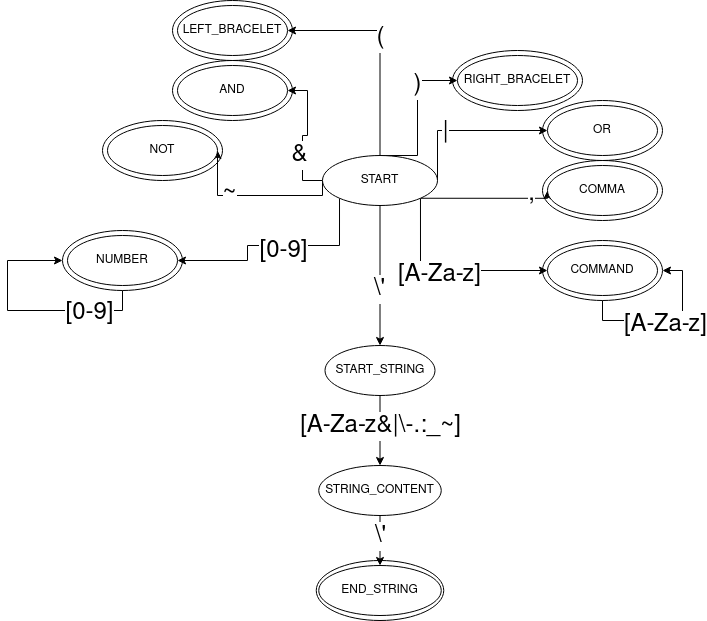
\includegraphics[scale=0.5]{obrazky-figures/RPQR_FSM.png}

\newpage

The lexical tokens that occur in RPQR language are:
\begin{itemize}
  \item left bracelet (
  \item right bracelet )
  \item and operator \&
  \item or operator |
  \item negation operator \textasciitilde
  \item number (consisting only of numeric characters e.g 123)
  \item string (hyphen separated string of alphanumeric and special characters e.g 'hello')
  \item command (command contains only alpha characters and has to be described by a~plugin e.g NAMELIKE)
  \item comma used mainly as a separator for command arguments ,
\end{itemize}

\subsection*{Syntactic analysis}
RPQR language syntactic analysis will be mainly precedent syntactic analysis because the language is statement-oriented. The precedent syntactic analysis uses an algorithm with a~symbol stack and acts accordingly to the precedent
syntactic table. This table defines what operators can be used at particular places and their respective
priorities. This solves the problem of evaluation of statements but there is still the matter of command
recognition and validation of argument types. Every command has to define what arguments it needs to work
properly. The initial configuration of RPQR will load commands and create context-free grammar for them.
Because every command has a different name and there is no need for dynamic arguments, a distinction should
be straightforward and effective.

Another more problematic matter is that for RPQR language to be able to handle all necessary use cases,
commands need to be able to accept the results of other commands as arguments. This is problematic since
it requires a new instance of precedent syntactic analysis to parse this statement. Fortunately, this
can be solved by cutting substatement out of the original statement and putting it queue of statements
that have to be yet parsed.

After all these problems are solved, RPQR will have an abstract syntactic tree containing all the information
that is necessary for the execution of statements e.g. commands that need to be executed first and operators
located in depth accordingly to their precedence. This tree will be later processed by semantic
analysis e.g. interpreter.

\newpage

Precedent syntactic table used for RPQR language:

\begin{center}
  \begin{tabular}{ |c|c|c|c|c|c|c| }
   \hline
     & ( & ) & \& & | & \textasciitilde & \$ \\
     \hline
  (  & < & = & <  & <  & <  & \#  \\
  \hline
  )  & \# & > & >  & >  & >  & >  \\  
  \hline
  \& & < & > & >  & <  & <  & >  \\
  \hline
  |  & < & > & <  & >  & <  & >  \\
  \hline
  \textasciitilde  & < & > & >  & >  & <  & >  \\
  \hline
  \$ & < & \# & <  & <  & <  & X \\
  \hline
  \end{tabular}
\end{center}

\textbf{Explanation of symbols}

The algorithm which handles syntactic analysis is driven by the precedent syntactic table. It always
looks at the first terminal symbol at the top of the stack and performs an operation that is specified
in the table by what symbol is in input.
\begin{itemize}
  \item < means that a special symbol marking the start of a particular statement needs to be put onto the stack and a new symbol loaded from the input
  \item = means only load new symbol
  \item > means that particular sub statements should be collapsed into one parent statement
  \item \# means that syntactic error occurred and provided input is not a valid RQPR language statement
  \item X marks the end of parsing of a valid RPQR language query
\end{itemize}

\subsection*{Semantic analysis}
Semantic analysis e.g. interpreter will be an implementation of a depth-first search algorithm for processing
of abstract syntactic tree provided by syntactic analysis. It is walking through the tree and putting
found nodes in a stack until it finds a command or statement that can be already resolved. When the command
that is defined by the accessible plugin is encountered, then the interpreter will filter loaded packages and
either provide them as the final result or use them as an operand to one of the operators.

When a command is executed or a statement can be evaluated accordingly to the type of operator that it
contains, part of the abstract syntactic tree related to it is marked as resolved and the temporary result
is saved into the appropriate node. This means that the final result will be present as the root
of the tree.

As in syntactic analysis, there is a problem with subsets used as an argument. These subsets have
to be executed similarly as they were processed into the abstract syntactic tree. When encountered
interpreter will stop command processing and proceed to resolve the substatement with higher priority.

\section{RPQR language and its use}
This section should provide usage examples of RPQR language and results that should be expected.
RPQR statement always consists of at least one command.

\subsection*{Simple command}

\textit{COMMAND()}

This command will receive the entire graph of packages as input and will be responsible for providing
a set of packages that conform to its filter. Since this command does not accept any arguments, as there
are no arguments supplied, the filter is static and can not be affected by the user.

There are currently no plugins providing such type of command.

\subsection*{Command with arguments}

\textit{ADVANCEDCOMMAND('package', 3)}

Command used like this accepts two arguments which alter his behavior. The first one is a~string
and the second is a number. RPQR language does not consider whitespace characters, so there is no
difference or problem with their presence in the query. Commands like this can have more advanced
behavior and are generally more useful than the ones without arguments.

Example of this type of command is: \textit{WHATDEPENDSON('libyang-1.0.225-1.fc34.x86\_64', 1)}

\subsection*{Command accepting subset as an argument}

\textit{SUBSETCOMMAND(NAMELIKE('cups'), 3)}

This is the most complex command that the RPQR language supports. This query will at first filter the
entire graph with the command \textit{NAMELIKE('cups')} and then supply its result to the \textit{SUBSETCOMMAND}
command. The second command will have the possibility to work with a subset and thus does not have to
work with the entire graph which results in an ability to work more efficiently or perform operations
with a specific context. For a~better explanation of how the query could work, here is an example.
The first command could gather packages that contain string \textit{cups} in their name. The second
could then filter only three first by their name in alphabetical order.

Example of this type of command is: \textit{SUBSETNAMELIKE('x86\_64', NAMELIKE('libyang'))}

\newpage

\subsection*{Operators}

\textbf{Intersection}

\textit{FIRSTCOMMAND() $\&$ SECONDCOMMAND()}

Operator \& can be used as an intersection between sets provided as outputs of two commands or sets.
Packages returned by query specified like this have to be present in both the left and right set.

\textbf{Join}

\textit{FIRSTCOMMAND() | SECONDCOMMAND()}

Operator | can be used to join sets provided by two commands or statements. It has a~lower priority
than intersection and means that resulting sets will contain packages that are present in either
left or right set of this statement.

\textbf{Negation}

\textit{\textasciitilde COMMAND()}

Operator \textasciitilde\space can be used to specify that the result set of packages can contain only such
packages that do not conform to conditions specified by \textit{COMMAND}. It is important
to keep in mind that the input of the command is always the entire graph.

\subsection*{Priorities of the operators}

When in need of complex conditions and a combination of commands, it is very useful to use bracelets
to force priority of evaluation and to avoid confusion between what the user expects as a result and
what is the real result. Without the bracelets, the standard priority is as follows:

\begin{itemize}
  \item \textasciitilde
  \item \&
  \item |
\end{itemize}

\textbf{Example of bracelet use:}

\textit{FIRSTCOMMAND() $\&$ SECONDCOMMAND() | THIRDCOMMAND()}

Explanation of this query is: return packages that conform to conditions of \textit{FIRSTCOMMAND}
and \textit{SECONDCOMMAND} or packages that conform to \textit{THIRDCOMMAND}. This is caused
by the priority of operators.

\textit{FIRSTCOMMAND() $\&$ (SECONDCOMMAND() | THIRDCOMMAND())}

This query looks very similar but some bracelets change their meaning very significantly.
Packages in result set has to conform to \textit{FIRSTCOMMAND} and to \textit{SECONDCOMMAND} or 
\textit{THIRDCOMMAND} in the same time. Bracelets allow us to form more complex descriptions of
packages that we are looking for.

\section{Plugin architecture and its interface}

Since the whole project will be written in Python which is an object-oriented language, all plugins
will be inherited from a class that will provide the standard interface expected by the RPQR project. There
should be an initialization method allowing the plugin to prepare helper structures and then a method responsible
for inserting information into the plugins. Packages have attributes and relationships, so there 
will have to be two types of plugins, one inserting proper attributes to nodes and another one that
will construct relationships between them. RPQR will work with attribute plugins as if they had
a higher priority so relationship plugins will be able to work with already prepared attributes and
there will be no unnecessary overhead.

Commands supplied by the plugin will also conform to the interface specified by their base class. Each
will have to list types of arguments that they need and implement a function that contains the logic of
their filtering operations. Since many commands will be working with similar graph algorithms such as
depth-first search or breadth-first search, the base class will provide an optimized implementation that
just needs specification of filter in a~form of function.

\section{Caching}

As was stated in the previous chapter, RPQR will need to use cache to save time consumed by building information
about packages contained in configured repositories. After careful consideration, the approach of
using JSON as a format of the cache was chosen. This way, even third-party tools will be able to manipulate
it and users will be able to read it if necessary. The cache will be invalidated only by users'
request to do so and when a new plugin is found. The presence of plugins will be tested by a special record
in the cache. Fortunately, all this is supported by the networkX library.

\section{API design}
RPQR needs to have a Python application programming interface so external developers can use its plugins
and features even more efficiently than through a command-line interface and create their solutions.
API will be using the same RPQR language as the command line interface and queries will be returning
NetworkX graphs. This way, applications using the API can walk through nodes that represent packages
and perform any transformation of the graph that they deem useful.

\newpage

\section{Command line interface design}
RPQR tool will be using one main positional option that has to be provided and that is a~query written
in RPQR language. By default, the output will go into standard output and log messages to standard error output.

The first two options that can, but do not have to be specified will be whether the user wants to see a visualization
of result created by his query and what attributes or relations should be included in the output.
Filtering of attributes and relations is helpful because, with multiple plugins, there can be a lot
of unnecessary data in the output that takes a lot of space. Another important option is the location
of the configuration file if the user does not want to use the default location which is \textit{/etc/rpqr.conf}.
The last option is whether the tool should invalidate the cache and build it again.

\chapter{Implementation and evaluation}
With research and design complete, the RPQR project can now be implemented in the best way possible.
This chapter will cover a deep description of the project's code and the algorithms it uses to fulfill the
assigned task. Each section will cover the limitations of the presented solution and what could be done
in the future to overcome them. Usage of the RPQR project will also be described in a form of a user
manual and a description of the way how new plugins are supposed to be developed using the RPQR interface.

\section{Important parts of implementation}
This section will show the most important parts of the implementation and structure of Python code.
Inheritance and general content of classes can be found on the class diagram.

\newpage

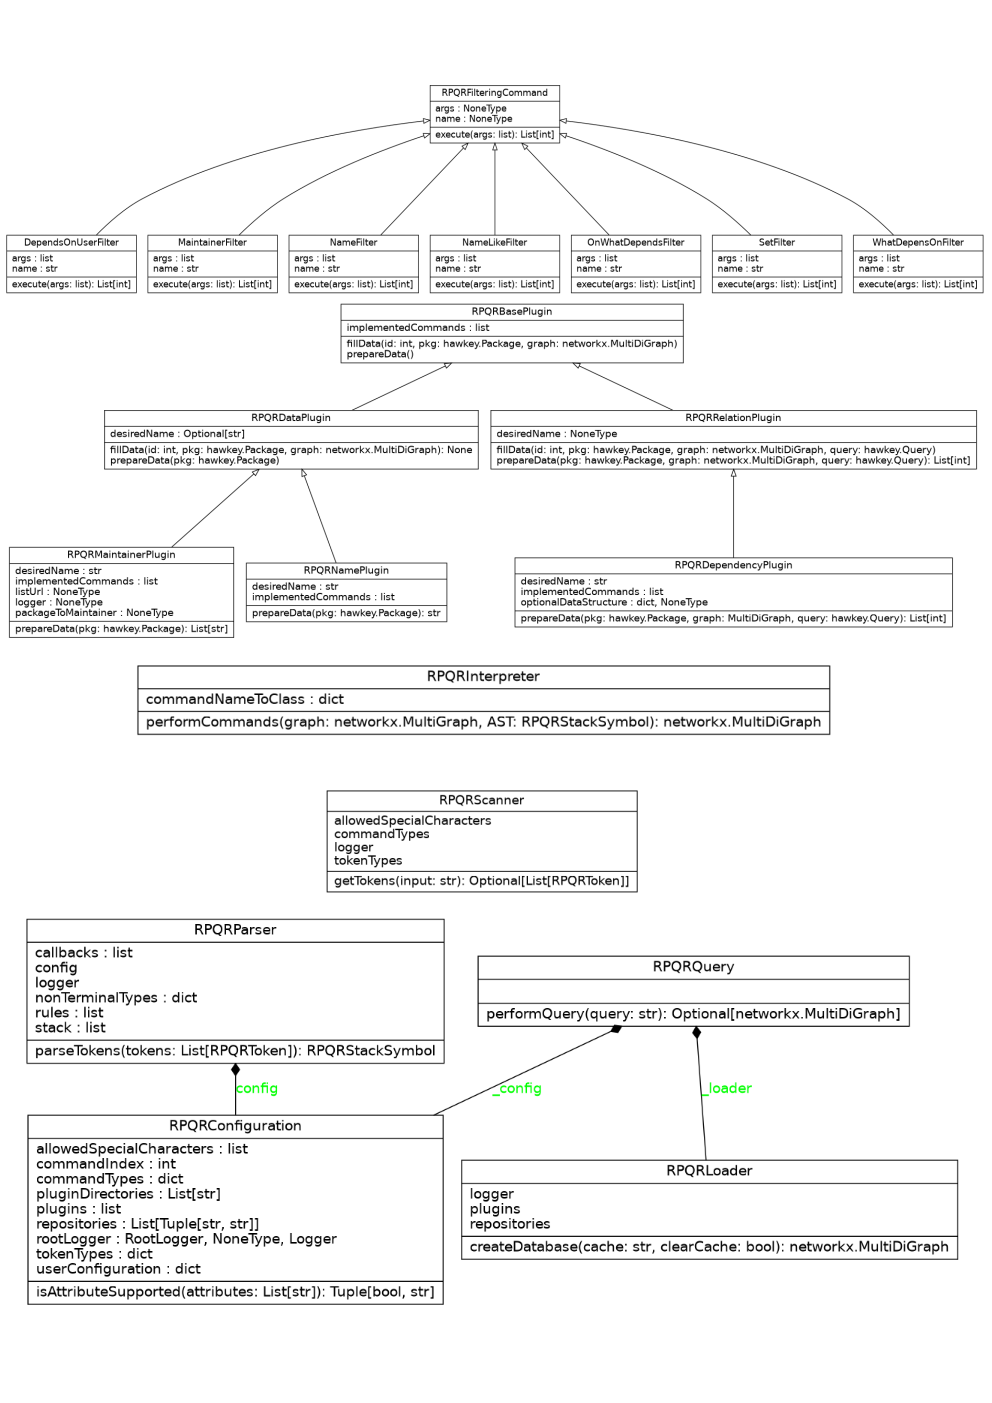
\includegraphics[scale=0.7]{obrazky-figures/class_diagram.png}

\subsection*{RPQRConfiguration}
RPQRConfiguration class serves for purposes of loading plugins and creating RPQR language structures
necessary for its successful parsing and interpreting. An instance of this class has to be created for
every use of the RPQR project and is used by all following components and their diverse operations.

\textbf{Initialization of plugins}

This is the centerpiece of plugin loading. The plugins are loaded by the following method, which walks through all configured directories
which according to configuration should contain plugin modules and if its file does not start with
an underscore then attempts to import them and create their instance. Two conditionals relate to the plugin configuration. The first one is checking whether a configuration related to
this plugin exists and thus should be provided to it and the second one is there for a case when
a user does not want to use the plugin at all, to save space for example, or to speed up processing.

\begin{lstlisting}
def _initializePlugins(self):
  """ Load plugins from supplied directories
  """
  for dir in self.pluginDirectories:
      sys.path.append(dir)
      pluginModules = os.listdir(dir)
      for file in pluginModules:
          moduleName = file[:-3]
          # if file name starts with _ then it is most likely not a plugin
          if moduleName.startswith("_"):
              continue
          cfg = None
          if moduleName in self.userConfiguration.keys():
              cfg = self.userConfiguration[moduleName]

          if (cfg != None and cfg.get("disabled") == "1"):
              self._logger.info(
                  "%s plugin was disabled in configuration" % moduleName)
              continue
          module = importlib.import_module(moduleName)
          pluginClass = getattr(module, moduleName)

          pluginInstance = pluginClass(rootLogger=self.rootLogger,
                                      config=cfg)
          self.plugins.append(pluginInstance)
\end{lstlisting}

\newpage

\subsection*{RPQRLoader}
RPQRLoader is a class responsible for the loading of data about packages through plugins and constructing
graph structures out of them. It is taking advantage of DNF API to retrieve the data as efficiently as
possible and access them in the same way as the package manager would.

\textbf{Construction of graph}

This method distinguishes between plugins that are supposed to add attributes to package nodes and
plugins that create relations between individual packages. The first kind is executed first so
relationship plugins can depend on them later. Each instance of the plugin has its fillData method
which is called for each package that was retrieved by DNF API. After the graph is built, a list
of plugins that were present during the creation of this structure is saved into the plugins list for easier
detection of invalid cache.

\begin{lstlisting}
def createDatabase(self, cache: str = None) -> NetworkX.MultiDiGraph:
  """ Get graph of packages with data and relations described by plugins
  :param cache: path to cache file, defaults to None
  :type cache: str, optional
  :return: Graph of packages
  :rtype: NetworkX.MultiDiGraph
  """
  graph = NetworkX.MultiDiGraph()
  dataPlugins = [plugin for plugin in self.plugins if isinstance(
      plugin, RPQRDataPlugin)]
  relationPlugins = [plugin for plugin in self.plugins if isinstance(
      plugin, RPQRRelationPlugin)]

  pluginRecords = []
  for plugin in dataPlugins + relationPlugins:
      pluginRecords.append((plugin, plugin.__class__.__name__))
  ...
  av_query = self._getAvailableQuery()
  q_avail = av_query.run()
  for id, pkg in enumerate(q_avail):
      graph.add_node(id)
      for pluginInstance in dataPlugins:
          pluginInstance: RPQRDataPlugin
          pluginInstance.fillData(id, pkg, graph)

  for id, pkg in enumerate(q_avail):
      for pluginInstance in relationPlugins:
          pluginInstance: RPQRRelationPlugin
          pluginInstance.fillData(id, pkg, graph, av_query)

  graph.graph["plugins"] = [name for (_, name) in pluginRecords]
  ...
  return graph
\end{lstlisting}

\subsection*{RPQRScanner}
RPQRScanner is a class responsible for scanning the query entered in RPQR language format. It is able
to recognize when there is a lexical error in the query and is used to parse a string into tokens.

\textbf{Implementation of finite state machine}

Method getTokens is responsible for creating a list of tokens out of input. It is composed of
a while cycle that parses characters and switches the state of the machine accordingly. It is strictly
implemented accordingly to the graph of FSM which was mentioned earlier.

\begin{lstlisting}
def getTokens(self, input: str) -> Optional[List[RPQRToken]]:
  ...
  while curInputIndex < len(input) + 1:
      if curInputIndex < len(input):
          c = input[curInputIndex]
      else:
          c = ''
      if curState == States.START:
          if c == '':
              break
          elif c == '(':
              curToken = RPQRToken(self.tokenTypes["leftBracelet"], c)
              curState = States.LEFTBRACELET
          elif c == ')':
              curToken = RPQRToken(self.tokenTypes["rightBracelet"], c)
              curState = States.RIGHTBRACELET
          elif c == '&':
              curToken = RPQRToken(self.tokenTypes["and"], c)
              curState = States.AND
          ...
          curInputIndex += 1
      elif curState == States.AND:
          tokens.append(curToken)
          curState = States.START
      elif curState == States.OR:
          tokens.append(curToken)
          curState = States.START
      elif curState == States.NUMBER:
          if c.isnumeric():
              curToken.appendToContent(c)
              curInputIndex += 1
          else:
              tokens.append(curToken)
              curState = States.START
\end{lstlisting}

\subsection*{RPQRParser}

RPQRParser is a class responsible for the processing of lexical tokens and the construction of abstract syntactic
trees that can be interpreted in a strictly defined way. The class contains helper methods for easier
manipulation with a list of tokens and methods considered as callbacks to certain operations encountered
in the source query. These operations are uses of operators like \textit{$\&$} or \textit{\textasciitilde}
which needs the abstract syntactic tree to be constructed in a~certain way.

\textbf{parsing algorithm}

\begin{lstlisting}
while True:
  while True:
      if curInput.type in self.config.commandTypes.values():
          commandRule = None
          for rule in self.rules[4:]:
              if rule[0] == curInput.type:
                  commandRule = rule
          childList = [curInput]
          for indexMember, member in enumerate(commandRule[1:]):
              if member == self.nonTerminalTypes["statement"]:
                ...
              if argToken.type != member:
                ...
              if (argToken.type in
                [self.config.tokenTypes["number"], self.config.tokenTypes["string"]]):
                  childList.append(argToken)
          newStatement = RPQRStackSymbol(
              self.nonTerminalTypes["statement"], childList)
          self.stack.append(newStatement)
          curInput = tokens.pop(0)
          continue

      lastTerminalIndex = 0
      ...

      requiredAction = precedencTable[self.stack[lastTerminalIndex].type][curInput.type]
      ...
  # decide whether we need to keep parsing or everything is already done
  if len(substatementQueue) == 0:
      return rootStatement
  else:
      curStatement = substatementQueue.pop(0)
      self.stack = [RPQRStackSymbol(self.config.tokenTypes["end"])]
      tokens = curStatement.children
      curInput = tokens.pop(0)
\end{lstlisting}

The parsing algorithm is based on the processing of a statement queue that contains all individual statements
that need to be parsed. The first cycle is going through a queue of statements and the inner one is
performing precedent syntactic analysis and calling appropriate callbacks. An interesting operation is
that when substatement is encountered (command accepts a statement as an argument) algorithm cuts this
substatement out of the source and inserts it into the queue for further resolution. Because of the tree's structure, it is possible to resolve the rest of the statement even when the construction of the substatement is not yet
known.

The current parsing algorithm is not able to handle commands that take a dynamic number of arguments. This
is a known limitation but because this feature was not needed in any relevant testing scenario,
RPQR will not at the time of this thesis contain such an option.

\newpage

\subsection*{RPQRInterpreter}

RPQRInterpreter is a class responsible for the interpretation of RPQR language. It is mainly composed out
of an algorithm that performs a depth-first search of the abstract syntactic tree and resolves nodes from
bottom to up direction.

\textbf{Interpretation algorithm}

\begin{lstlisting}
while len(stack) > 0:
    curNode = stack[-1]
    curResult = resultStack[-1]
    if curNode.operator is not None:
        if len(curResult.childResults) < 1:
            ...
        elif curNode.operator != '~' and len(curResult.childResults) < 2:
            ...
        else:
            # now we have all operands, we can begin resolution
            validNodes = []
            ...
            stack.pop()
            resultStack.pop()
    else:
        ...
        notResolvedStatementFound = False
        for argIndex, argType in enumerate(commandClass.args):
            if argType == str or argType == int:
                # literals can be resolved right away
                if (argIndex > len(curResult.childResults)-1):
                    curResult.childResults.append(RPQRResultTree(
                        curNode.children[1:][argIndex].content, []))
                else:
                    continue
            elif argType == list:
                if (argIndex > len(curResult.childResults)-1):
                    ...
                    break
                else:
                    continue
        if notResolvedStatementFound:
            continue
        arguments = []
        for partResult in curResult.childResults:
            arguments.append(partResult.result)
        curResult.result = commandClass.execute(graph, arguments)
        stack.pop()
        resultStack.pop()
\end{lstlisting}

The algorithm distinguishes between nodes that represent statements composed out of operator and operands
and commands that filter packages. Processing of such nodes differs because operators are built-in
and have a fixed number of arguments while commands are defined by plugins and every command can have
a different number of arguments. The algorithm walks through the abstract syntactic tree and performs partial
operations by calling execute method of plugins with already loaded arguments. When the root node
is reached by resolution and its result is known, then the result can be returned by \textit{performCommands}
method and formated by users' requirements.

\newpage

\subsection*{RPQR script}
RPQR script is a command-line utility that allows users to use the RPQR project comfortably. It is designed
to take advantage of the whole project and its features while providing the user with the ability to
control for example when a cache file should be invalidated and overwritten.

\textbf{RPQR script implemenation}

\begin{lstlisting}
  rpqrcfg = RPQRConfiguration(pluginDirectories, namexrepository, cfgParser)
  loader = RPQRLoader(rpqrcfg)
  graph = loader.createDatabase(cacheFile, args.clearcache)
  # we will not be performing empty query
  if len(args.query) == 0:
      sys.exit(0)
  result = RPQRQuery.performQuery(args.query, graph, rpqrcfg)
  if result is None:
      sys.exit(1)
  # we will filter result attributes according to supplied parameters
  if len(args.filterattributes) != 0 or len(args.filterrelations) != 0:
      ...
      if len(args.filterattributes.split(";")[0]) != 0:
          for node in result.nodes:
              for key in list(result.nodes[node].keys()):
                  if not key in args.filterattributes.split(";"):
                      del result.nodes[node][key]
      if len(args.filterrelations.split(";")[0]) != 0:
          for node in result.nodes:
              for u, v, edge_key in graph.out_edges([node], keys=True):
                  if not edge_key in args.filterrelations.split(";"):
                      graph.remove_edge(u, v, key=edge_key)
  # if result should not be visualized then just print it
  # in JSON format to stdout
  if not args.visualize:
      print(json.dumps(json_graph.node_link_data(
          result), indent=4, sort_keys=True))
      sys.exit(0)

  # labeling requires some more processing
  ...
  pos = NetworkX.spring_layout(result)
  NetworkX.draw_NetworkX(result, pos=pos, with_labels=True, labels=labelDict)
  edgeLabels = dict([((n1, n2), key) for n1, n2, key in result.edges])
  NetworkX.draw_NetworkX_edge_labels(result, pos=pos, edge_labels=edgeLabels)
  plt.show()
\end{lstlisting}

Implementation of RPQR script uses RPQR API and allows users to specify whether the result should be
visualized or printed out through the standard output. Another very useful feature is the filtering of
attributes and relations that should be included in the output. The script is using matplotlib Python
library to render graphs of packages if required.

\section{User manual}
This section contains a manual of the RPQR tool and a detailed description of the way how it is intended to be
used. Another part provides information about the development of plugins and scripts that are using RPQR
API to retrieve and filter package metadata.

\textbf{NAME}

RPQR - RPM package query resolver

\textbf{SYNOPSIS}

RPQR [-h] [-{}-cfgpath <CFGPATH>] [-{}-filterattributes <FILTERATTRIBUTES>] \newline
[-{}-filterrelations <FILTERRELATIONS>] [-{}-visualize] [-{}-clearcache] <QUERY>

\textbf{DESCRIPTION}

RPQR utility is supposed to make querying RPM repositories about package metadata easy by providing
the user with the means to filter them by such metadata and individual types of relations that occur between
them. Utility is configurable through configuration file which is located by default in \textit{/etc/rpqr.conf}.

\textbf{OPTIONS}

\begin{itemize}
  \item -h, -{}-help
    \subitem Show help message and exit
  \item -{}-cfgpath <CFGPATH>
    \subitem Path to configuration file
  \item -{}-filterattributes <FILTERATTRIBUTES>
    \subitem Specify list of attributes which interest you in the result. If left empty, then all attributes will be present in result
  \item -{}-filterrelations <FILTERRELATIONS>
    \subitem Specify list of relations which interest you in the result. If left empty, then all relations will be present in result
  \item -{}-visualize
    \subitem Visualize result
  \item -{}-clearcache
    \subitem Clear cache
\end{itemize}

\textbf{CONFIGURATION FILE}

The following configuration file should illustrate general principles of how the RPQR utility behavior
can be changed with it.

\begin{lstlisting}
[RPQR]
pluginDirectories=["./rpqr/loader/plugins/implementations"]
cache=/var/tmp/rpqr.json

[RPQRRepo_f34-repo]
url=http://ftp.fi.muni.cz/pub/linux/fedora/linux/releases/34/Everything/x86_64/os/

[RPQRMaintainerPlugin]
url=https://src.fedoraproject.org/extras/pagure_owner_alias.json
\end{lstlisting}

The first section named \textit{RPQR} is the main configuration section that contains the most important
setting. \textit{pluginDirectories} is an array of directories that contain Python modules with RPQR
plugins. \textit{cache} is the path to the cache file, when this path is not supplied then RPQR utility
will not use cache.

The second section named \textit{RPQRRepo\_f34-repo} is meant to set up the repository that which user wants to
query. There can be one to n number of repositories and they all have to be configured in their 
section with prefix \textit{RPQRRepo\_} and member URL which specifies the base URL of the repository.

The third section is required for \textit{RPQRMaintainerPlugin}. Each plugin can have its section
of configuration and member disabled, which when set to \textit{1} will prevent this plugin from
working. Plugin configuration is described by plugins individually and is mentioned here only for
the clarification of examples.

\textbf{Example of use}

RPQR "ONWHATDEPENDS('libyang-1.0.225-1.fc34.x86\_64', 1)" -{}-filterattributes "name" -{}-filterrelations "depends" -{}-visualize

\textbf{RPQR language}

RPQR language serves as a means to specify what packages the user wants to see in the result. Take advantage
of operators to create an appropriate combination of commands to get the results that you want.

\newpage

\textbf{Operators}

\begin{itemize}
  \item \& - package has to conform to both right and left statements
  \item  | - package has to conform to either left or right statements
  \item  \textasciitilde - package must not conform to statement located on the right 
\end{itemize}

\textbf{Parenthesis}

RPQR also supports parenthesis to provide further means to set the priority of statements that are specified.
Use parenthesis to make your query more readable and to make sure that the result is what you expect.
\textit{statement1 $\&$ (statement2 | statement3)} This statement is not equal to the version without
parenthesis specified like this \textit{statement1 $\&$ statement2 | statement3}. The semantic of the first
statement is: \textbf{Find packages that conform to statement1 and at the same time conform to either
statement2 or statement3}. On the other hand, the second statement meaning is: \textbf{Find packages
that conform to both statement1 and statement2 but if the package conforms to statement3 then it does not
have to conform either to statement1 or statement2}.

\newpage

\textbf{Official distributed plugins documentation}

This section of the manual contains documentation about the behavior of plugins that are officially
distributed with the RPQR tool and supported by the maintainers.

\textbf{RPQRNamePlugin}

RPQRNamePlugin is one of the most important plugins for RPQR utility. It gathers the complete name of the
package, meaning its name, version, release, and architecture. It is an attribute plugin and inserts
attribute \textit{name} into the package.

\begin{itemize}
  \item Added attribute: 'name'
  \item Added commands: 'NAME', 'NAMELIKE', 'SUBSETNAMELIKE'
  \item Depends on plugins: None
\end{itemize}

\textbf{Commands provided by RPQRNamePlugin}

\textbf{NAME}

Required arguments: name (string literal)

\textit{NAME} command filters out only package that has the same name attribute as was specified
with the name argument.

Example of use: \textit{NAME('libyang-1.0.225-1.fc34.x86\_64')}

\textbf{NAMELIKE}

Required arguments: name (string literal)

\textit{NAMELIKE} command filters out packages that contain substring specified with the argument
\textit{name}.

Example of use: \textit{NAMELIKE('libyang')}

\newpage

\textbf{SUBSETNAMELIKE}

Required arguments: name (string literal), statement (RPQRLanguage statement)

\textit{SUBSETNAMELIKE} command filters out packages returned by argument \textit{statement} that
contain substring specified with the argument \textit{name}.

Example of use: \textit{SUBSETNAMELIKE('x86\_64', NAMELIKE('libyang'))}

Explanation of the example semantics: This query returns packages that contain \textit{libyang} in their
name and at the same time \textit{x86\_64} substring. The difference between this statement and
\textit{NAMELIKE('x86\_64') \& NAMELIKE('libyang')} is that the first query will be faster because
it has to go through an only subset of packages.

\textbf{RPQRDependencyPlugin}

RPQRDependencyPlugin is a relation plugin that gathers information about package dependencies and
creates dependency relations between nodes that represent them in the RPQR graph of packages.

\begin{itemize}
  \item Added relation: 'depends'
  \item Added commands: 'ONWHATDEPENDS', 'WHATDEPENDSON'
  \item Depends on plugins: RPQRNamePlugin
\end{itemize}

\textbf{Commands provided by RPQRDependencyPlugin}

\textbf{ONWHATDEPENDS}

Required arguments: name (string literal), depth (numeric literal)

\textit{ONWHATDEPENDS} command filters out packages on which package, with name attribute matching
\textit{name} argument, depends. \textit{depth} argument is controlling the depth to which RPQR
should go when gathering dependencies from the graph. Depth zero means that only the package specified
by name will be present in the output, value one causes that only direct dependencies will be present, and
so on.

Example of use: \textit{ONWHATDEPENDS('libyang-1.0.225-1.fc34.x86\_64', 1)}

\textbf{WHATDEPENDSON}

Required arguments: name (string literal), depth (numeric literal)

\textit{WHATDEPENDSON} command filters out packages that depend on the package, with name attribute matching
\textit{name} argument. \textit{depth} argument is controlling the depth to which RPQR
should go when gathering dependent packages from the graph. Depth zero means that only the package specified
by name will be present in the output, value one causes that only directly dependent packages will be present, and
so on.

Example of use: \textit{WHATDEPENDSON('libyang-1.0.225-1.fc34.x86\_64', 1)}

\textbf{RPQRMaintainerPlugin}

RPQRMaintainerPlugin is an attribute plugin that gathers information about maintainers who work
on packages. It inserts attribute \textit{maintainer} into packages. Plugin, unfortunately, depends
on the format of the list of maintainers which has to be in JSON.

\begin{itemize}
  \item Added attribute: 'maintainer'
  \item Added commands: 'MAINTAINER', 'DEPENDSONUSER'
  \item Depends on plugins: RPQRDependencyPlugin
\end{itemize}

\textbf{Commands provided by RPQRMaintainerPlugin}

\textbf{MAINTAINER}

Required arguments: maintainers name (string literal)

\textit{MAINTAINER} command filters out packages that have a maintainer specified with the argument
maintainers name in the list of their maintainers.

Example of use: \textit{MAINTAINER('tkorbar')}

\textbf{DEPENDSONUSER}

Required arguments: maintainers name (string literal), depth (numeric literal)

\textit{DEPENDSONUSER} command filters out packages that depend on the work of the maintainer specified with
argument \textit{maintainers name}. That means that depth zero will retrieve packages that have specified
maintainer in the list of its maintainers as \textit{MAINTAINER} command would. Values higher than zero
will retrieve packages that depend on those retrieved with depth zero.

Example of use: \textit{DEPENDSONUSER('tkorbar', 1)}

\textbf{RPQRMaintainerPlugin configuration}

RPQRMaintainerPlugin has one additional variable for configuration not included in the default setting for
all plugins. It is a variable URL that specifies the location of the maintainer list.

Example:
\begin{lstlisting}
[RPQRMaintainerPlugin]
url=https://src.fedoraproject.org/extras/pagure_owner_alias.json
\end{lstlisting}

\textbf{LICENSE}

You may copy, distribute and modify the software as long as you track changes/dates in source files.
Any modifications to or software including (via compiler) GPL-licensed code must also be made available
under the GPL along with build \& install instructions.

\section{API documentation and example of scripting}

RPQR project allows developers to create their plugins which can further extend its ability to
recognize attributes and relations between packages. This section will show already existing plugins
on which it will describe plugin development and the importance of individual parts.

\subsection*{RPQRMaintainerPlugin}

\begin{lstlisting}
  class RPQRMaintainerPlugin(RPQRDataPlugin):
    """ Plugin allowing us to store information about package maintainers
        and ask Queries about them
    """
\end{lstlisting}

Plugin which wants to add a new attribute to packages needs to inherit from RPQRDataPlugin class.
Please pay attention to the file name of your Python module. The filename has to be the same as
the name of the class.

\begin{lstlisting}
    desiredName = "maintainer"

    implementedCommands = [MaintainerFilter, DependsOnUserFilter]
\end{lstlisting}

\textit{desiredName} is the name of the attribute that this plugin wants to add. \textit{implementedCommands}
is a list of classes of commands that this plugin wants to add to the RPQR project. Commands will be described
later.

\begin{lstlisting}
    packageToMaintainer = None

    def __init__(self, rootLogger: Logger = None, config: dict = None):
        self.listUrl = None
        if config == None and rootLogger != None:
            lgr = rootLogger.getChild("RPQRDataPlugin")
            lgr.warning("url for retrieval of maintainers was not supplied")
            return

        self.logger = rootLogger.getChild(
            "RPQRDataPlugin") if rootLogger != None else None

        self.listUrl = config.get("url")
\end{lstlisting}

\textit{packageToMaintainer} is a helper class variable. A~plugin can declare its variables as it sees
fit. The plugin needs to be ready for use-cases when it does not has access to logger or configuration
and has to act accordingly. Because \textit{RPQRMaintainerPlugin} needs to know the URL for retrieval
of the maintainer list, it has to access configuration. All such use cases have to be documented.

\newpage

\begin{lstlisting}
    def _downloadJson(self):
        if self.listUrl == None:
            return {}
        receivedResponse = requests.get(self.listUrl)

        if receivedResponse.status_code != 200:
            self.logger.error(
                "RPQR was unable to retrieve maintainer list from supplied url %s" % self.listUrl)

        return receivedResponse.json().get("rpms", {})
\end{lstlisting}

This is a helper method for retrieval of the maintainer list. Plugins can access any source of information
that they want but this also has to be documented.

\begin{lstlisting}
    def prepareData(self, pkg: hawkey.Package) -> List[str]:
        """Get maintainers of package

        :param pkg: hawkey package information
        :type pkg: hawkey.Package
        :return: list of maintainers
        :rtype: List[str]
        """
        # download package maintainer list and build dictionary from it
        if RPQRMaintainerPlugin.packageToMaintainer is None:
            RPQRMaintainerPlugin.packageToMaintainer = {}
            data = self._downloadJson()
            data: dict
            for name, value in data.items():
                RPQRMaintainerPlugin.packageToMaintainer[name] = value
        # owner alias json uses source names as keys
        return RPQRMaintainerPlugin.packageToMaintainer[pkg.name if pkg.source_name == None else pkg.source_name]
\end{lstlisting}

\textit{prepareData} is called for each package and has to return a value that should be
saved to the implemented attribute. If block is there because the first run of this method will retrieve
a list of maintainers and create a helper dictionary to accelerate loading. Please use such approaches
to keep the project fast. After such initialization, every package is just returned a list of maintainers
from \textit{packageToMaintainer} dictionary. The ternary operator is there because source packages
have different naming conventions in DNF API than the binary ones and RPQR has to be ready for both.

\newpage

\subsection*{DependsOnUserFilter}

\begin{lstlisting}
  class DependsOnUserFilter(RPQRFilteringCommand):
    """Command allowing filtering packages which depend on certain maintainer.
    That means the person is either maintaining them or package depends on
    package which they maintain recursively.
    """
    args = [str, int]
    name = "DEPENDSONUSER"

    def execute(graph: NetworkX.MultiDiGraph, args: list) -> List[int]:
        """ Get list of ids of packages which depend on user specified in args[0]
        to max depth args[1]

        :param graph: built graph of packages
        :type graph: MultiDiGraph
        :param args: arguments supplied to command
        :type args: list
        :return: node ids of packages which depend on specified maintainer
        :rtype: List[int]
        """
        targetUser = args[0]
        depth = int(args[1])
        nodes = [a for a in list(graph.nodes)
                 if targetUser in graph.nodes[a]["maintainer"]]

        return RPQRFilteringCommand._BFS(graph, nodes, depth, "depends")
\end{lstlisting}

This is a more complex command out of \textit{RPQRMaintainerPlugin}s two commands so it is more worthy of
explanation. All commands have to inherit from \textit{RPQRFilteringCommand} class and declare \textit{args}
array and \textit{name} class variable. \textit{args} is an array that tells the RPQR project what arguments
this command needs. Allowed types are str, int and list. Str means string literal, int means numeric
literal and list is a result of substatement. A~list is handled as a list of integers. \textit{name}
is the name of the command used to invocate it.

All commands have to implement \textit{execute} method. \textit{execute} method receives a built graph
of packages and their arguments. As you can see, the first command gathers the ids of nodes that have specified
maintainers in their maintainer list. Ids are then passed to static method \_BFS which is a prepared
implementation of Breadth-First Search. Breadth-First Search then finds dependent nodes to the specified
depth.

\newpage

\subsection*{RPQRDependencyPlugin}

\begin{lstlisting}
  class RPQRDependencyPlugin(RPQRRelationPlugin):
    """Plugin for gathering dependencies of packages and allowing filtering
    by them
    """
    desiredName = "depends"
    implementedCommands = [OnWhatDependsFilter, WhatDepensOnFilter]

    def __init__(self, rootLogger: Logger = None, config: dict = None) -> None:
        self.optionalDataStructure = None

    def prepareData(self, pkg: hawkey.Package, graph: MultiDiGraph, query: hawkey.Query) -> List[int]:
        """ Get list of nodes to which we want to form this relation

        :param pkg: hawkey package object. Holds information supplied by dnf api
        :type pkg: hawkey.Package
        :param graph: graph of packages
        :type graph: MultiDiGraph
        :param query: hawkey query object. Allows further queries through dnf api
        :type query: hawkey.Query
        :return: list of target nodes for this node
        :rtype: List[int]
        """
        # we will use dictionary for optimalization of this process
        if self.optionalDataStructure == None:
            self.optionalDataStructure = {}
            for (node, attribs) in graph.nodes.items():
                self.optionalDataStructure[attribs["name"]] = node

        edges = list()
        requiredPackages = query.filter(provides=pkg.requires).run()
        for dependency in requiredPackages:
            target = self.optionalDataStructure[str(dependency)]
            edges.append(target)
        return edges
\end{lstlisting}

Relation plugins are very similar to those adding attributes with a few differences. Relation plugins
can access a graph of packages that they can access and Hawkey query from DNF API. Relation
plugins are returning a list of target nodes of oriented edges that they are creating.

\section{Use of RPQR API to perform queries}

Working of RPQR API will be described on the \textit{RPQROrphaned} script which was used for testing
of RPQR project.

\begin{lstlisting}
  if __name__ == "__main__":
    # set up configuration
    config = RPQRConfiguration([os.path.dirname(rpqr.loader.plugins.implementations.__file__)],
                               [("fedora-repo", "http://ftp.fi.muni.cz/pub/linux/fedora/linux/releases/33/Everything/x86_64/os/"),
                                ("source-repo", "http://ftp.fi.muni.cz/pub/linux/fedora/linux/releases/33/Everything/source/tree/")],
                                {"RPQRMaintainerPlugin":{"url": "https://src.fedoraproject.org/extras/pagure_owner_alias.json"}})
    query = RPQRQuery(config)
    result = query.performQuery("MAINTAINER('orphan')")
    for node in list(result.nodes):
        # now we will recursively gather packages which depend on every orphaned package
        dependentPackages = query.performQuery(
            "WHATDEPENDSON('%s', 20)" % result.nodes[node]["name"])
        # get maintainers affected by this change
        maintainerList = []
        for pkgId in list(dependentPackages.nodes):
            for maintainer in dependentPackages.nodes[pkgId]["maintainer"]:
                if maintainer not in maintainerList:
                    maintainerList.append(maintainer)
        maintainerList = list(dict.fromkeys(maintainerList))
        # orphan is just a placeholder so remove it
        maintainerList.remove('orphan')
        print("%s => " % dependentPackages.nodes[node]["name"], end="")
        for maintainer in maintainerList:
            print("%s " % maintainer, end="")
        print()
\end{lstlisting}

Every use of the API needs to start with creating an instance of \textit{RPQRConfiguration} class.
After that, the only other required thing is an instance of \textit{RPQRQuery} class and then it is
possible to create perform queries. Results are returned as a \textit{NetworkX} graph and have to be
worked with as. This script walks through orphaned packages and finds other maintainers affected by
their orphaning. 

\section{Testing}

To ensure that the RPQR project is maintainable, testing is needed. Since the RPQR codebase is written
in a way that allows dividing the project into individually functional blocks, it is possible to test
each part of it separately. The structure of the tests copies the structure of the source code.
All tests use \textit{unittest}\cite{unittest} Python module which provides functions necessary for testing and
supports automatic discovery which can be executed with the command: python3 -m unittest discover -p "Test*" -s ./test/.

For each significant class in the RPQR project, there is a test case that contains several tests for
individual features. Since test cases are similar, the principle of this technique will be illustrated
in one of those cases which is the most complicated one.

\subsection*{Test case description}

The following test case is meant to verify that the RPQRParser can parse tokens prepared by the RPQRScanner
and create an abstract syntactic tree out of them. This should be isolated from the implementation
of any plugins, and thus mock plugins were created\footnote{\textit{Mock} means that a component just acts like
its true implementation but contains only parts that are relevant for testing}. Mock plugins are loaded
into the configuration and provide simple commands.

The first test is a test of parsing a simple call of a command. The abstract syntactic tree produced by
the parser has to be identical to the one manually constructed according to the way how the algorithm
should work. The second test is performing a similar task but tokens are prepared as if a statement
with $\&$ operator was supplied in the query.

The third test is a result of the development cycle after the first release of the RPQR project. An issue
with the parsing of statements supplied as arguments was discovered and fixed. To prevent any future
regression, the problem was fixed with a commit containing documentation about it and this test can verify
that this problem will not be re-introduced in any of the future releases. This approach is very
useful and should be enforced on any future contributions or new features since it allows the project
to be tested for real problems and extends test coverage.

The complete test suite is available on the attached medium in the folder \textit{test}.

\newpage

\begin{lstlisting}
  class TestRPQRParser(unittest.TestCase):
    def testParserOne(self):
        config = RPQRConfiguration(
            ["./test/query/language/parser/mock_plugins"], [])
        parser = RPQRParser(config)
        mylist = [...]

        structure = parser.parseTokens(mylist)
        mystruct = RPQRStackSymbol(
            16, [RPQRToken(13, "DUMMY"), RPQRToken(6, "argument")])
        self.assertEqual(structure, mystruct)

    def testParserTwo(self):
        config = RPQRConfiguration(
            ["./test/query/language/parser/mock_plugins"], [])
        parser = RPQRParser(config)
        mylist = [...]

        structure = parser.parseTokens(mylist)
        mystruct = RPQRStackSymbol(16, [RPQRStackSymbol(16, [RPQRToken(13, "DUMMY"), RPQRToken(
            6, "argument")]), RPQRStackSymbol(16, [RPQRToken(13, "DUMMY"), RPQRToken(6, "argument2")])], "&")
        self.assertEqual(structure, mystruct)

    def testSubstatementParsing(self):
        config = RPQRConfiguration(
            ["./test/query/language/parser/mock_plugins"], [])
        parser = RPQRParser(config)

        mylist = [...]

        structure = parser.parseTokens(mylist)
        mystruct = RPQRStackSymbol(16, [RPQRToken(15, "SUB"), RPQRStackSymbol(16, [RPQRStackSymbol(16, [RPQRToken(13, "DUMMY"), RPQRToken(
            6, "argument")]), RPQRStackSymbol(16, [RPQRToken(13, "DUMMY"), RPQRToken(6, "argument2")])], "&")])
        self.assertEqual(structure, mystruct)
\end{lstlisting}

\newpage

\section{Distribution}

The RPQR project is distributed through a Python package which can be installed with the pip\cite{pip} tool.
At the moment of release 1.0.1, it is possible to install it from the source directory with the pip
tool or use the RPM package. RPM package is provided by a public repository hosted on Fedora copr\footnote{https://copr.fedorainfracloud.org/coprs/tkorbar/RPQR/}
website. The package is built according to the spec file located in the source root directory.
It uses prepared packaging macros and with them can install the project with the pip tool so
installation is even more centralized and simplified. Every build also discovers and executes the tests.

\begin{lstlisting}
%prep
%setup -q -n RPQR

%generate_buildrequires

%build
%pyproject_wheel

%install
sed -i "s;\\./rpqr/loader/plugins/implementations;%{python3_sitelib}/rpqr/loader/plugins/implementations;g" example.conf
mkdir -m 0755 -p %{buildroot}/%{_sysconfdir}
install -m 0644 -vp example.conf            %{buildroot}/%{_sysconfdir}/rpqr.conf
mkdir -m 0755 -p %{buildroot}/%{_mandir}/man1/
install -m 0644 -vp RPQR.1                  %{buildroot}/%{_mandir}/man1/
%pyproject_install

%check
python3 -m unittest discover -p "Test*" -s ./test/
\end{lstlisting}

The \textit{setup.py} script which uses Python setup tools is very simple but it fulfills its purpose and
handles installation of project modules to their appropriate directories.

\begin{lstlisting}
setup(name='rpqr',
    version='1.0.1',
    description='RPM package query resolver',
    author='Tomas Korbar',
    author_email='tkorbar@redhat.com',
    packages=find_packages(exclude=["test.*", "test"]),
    scripts=["bin/RPQROrphaned", "bin/RPQR"]
    )
\end{lstlisting}

\section{Evaluation}

RPQR projects' usefulness was evaluated with the \textit{RPQROrphaned} script mentioned earlier in
the API documentation. The previous solution needed tens of minutes to create a list of orphaned packages
and maintainers that are affected, \textit{RPQROrphaned} script needs one minute on a system with a casual processor.

There are results measured with the Linux time command when \textit{RPQROrphaned} is compared with
\textit{find\_unblocked\_orphans.py}\cite{orphans}
script developed for the same purpose by Miroslav Hroncok with previously accessible technologies.

\textbf{find\_unblocked\_orphans.py}

\begin{lstlisting}
real  12m32.938s
user  2m37.206s
sys 0m2.847s  
\end{lstlisting}

\textbf{RPQROrphaned}

\begin{lstlisting}
real  0m30.988s
user  0m25.159s
sys 0m0.910s
\end{lstlisting}

\chapter{Conclusion}

The RPQR project proved that the problem with query resolution about various metadata of packages can
be solved properly. The script that now performs tasks that were present in the past is faster than the
previous solutions and the project is ready to adapt to various new tasks that can occur in the future.

All initial goals of this thesis were fulfilled and the project is ready for further development because
of well-documented code and set of tests that can always verify whether new changes did not create a
regression.
